\documentclass[11pt,a4paper]{ctexart}
\usepackage[margin=2.2cm]{geometry}
\usepackage{graphicx}
\usepackage{booktabs}
\usepackage{longtable}
\usepackage{array}
\usepackage{amsmath}
\usepackage{hyperref}
\usepackage{xcolor}
\usepackage{fancyhdr}
\usepackage{enumitem}
\usepackage{float}
\usepackage{caption}

\setlist[itemize]{leftmargin=2em,itemsep=0.2em,topsep=0.3em}
\setlist[enumerate]{leftmargin=2em,itemsep=0.2em,topsep=0.3em}

\hypersetup{
  colorlinks=true,
  linkcolor=blue!50!black,
  urlcolor=blue!60!black
}

\pagestyle{fancy}
\fancyhf{}
\setlength{\headheight}{14pt}
\lhead{实验软件操作说明书}
\rhead{2026-07-05}
\cfoot{\thepage \quad / \quad \url{https://github.com/Es777777/485experiment-software-portable}}
\rfoot{}

\title{\textbf{实验软件操作说明书}\\v1.0.4 便携版细化操作版\\
\large 维护者邮箱：\texttt{koji3527@qq.com}\quad (每日上限 8 封，间隔 60 秒)\\
\large 项目主页：\url{https://github.com/Es777777/485experiment-software-portable}}
\author{}
\date{2026 年 10 月 13 日}

\begin{document}
\maketitle
\tableofcontents
\newpage

\section{说明}

本文档面向日常实验操作，重点回答四类问题：

\begin{enumerate}[leftmargin=2em]
  \item 软件从哪里启动，先看哪里；
  \item 实时曲线怎么判断是否正常；
  \item PWM 分组测量应该按什么顺序做；
  \item 遇到曲线异常、重量不对、导出不对时先查什么。
\end{enumerate}

本文档基于当前已核对的远端最新主线版本整理：
\begin{itemize}[leftmargin=2em]
  \item GitHub 远端主线：\texttt{origin/main}
  \item 当前发布版本：\texttt{v1.0.4}
  \item 便携版压缩包：\texttt{485experiment-software-portable-v1.0.4-20261013.zip}
  \item 反馈邮箱：\texttt{koji3527@qq.com}（每日上限 8 封，间隔 60 秒）
\end{itemize}

\section{软件组成}

\subsection{主要入口}

\begin{itemize}[leftmargin=2em]
  \item 启动器：\texttt{app\_launcher.py} 或便携版中的 \texttt{实验软件.exe}
  \item 实时曲线与分组测量主脚本：\texttt{scripts/serial\_logger\_with\_plot.py}
  \item 普通采集日志：\texttt{logs/}
  \item 分组测量导出结果：\texttt{output/}
  \item 串口和寄存器配置：\texttt{config/logger\_config.json}
\end{itemize}

\subsection{你实际会接触到的两个窗口}

\begin{enumerate}[leftmargin=2em]
  \item 启动器主界面：选择配置、确认串口、启动实时曲线；
  \item 实时曲线窗口：观察 ch1/ch2/ch3 与 total\_force，执行去皮、开始测量、结束测量、下一组、导出表格。
\end{enumerate}

\section{启动前检查}

\subsection{串口选型（双 COM）与设备管理器排查}

本软件需要\textbf{两路独立的 USB 串口}（v1.0.4 新增）。开始前请先把硬件
接好，再在系统层面确认每路串口实际对应的 COM 编号。

\subsubsection{两个 COM 口的区别}

\begin{itemize}[leftmargin=2em]
  \item \textbf{485 采集串口}：连 RS485 总线，读取 ch1/ch2/ch3 重量寄存器；
  \item \textbf{PWM 输出串口}：连 PWM 控制器（USB 转 TTL），用于写 PWM 值；
  \item 两路可以接同一台物理机器的不同 USB 口，分别在设备管理器里识别为
        不同的 COM 编号；
  \item 如果 PWM 控制器和 485 设备是同一台（功能码 06 写在 485 总线寄存器 100），
        可以不填 PWM 串口，程序会自动回退到用 485 串口写。
\end{itemize}

\subsubsection{怎么在设备管理器里找 COM 编号}

\begin{enumerate}[leftmargin=2em]
  \item 把两路 USB 串口都插到电脑；
  \item 右键“此电脑” $\rightarrow$ “管理” $\rightarrow$ “设备管理器”；
  \item 点开“端口 (COM \& LPT)”；
  \item 把 485 串口拔下，看哪个条目消失，记下它的 COM 编号（例如
        \texttt{USB-SERIAL CH340 (COM3)}）；
  \item 再插上，拔下 PWM 串口，同样记下 COM 编号（例如
        \texttt{USB-SERIAL CH340 (COM5)}）；
  \item 回到启动器，在 “Modbus” 页签依次选择两个 COM 口。
\end{enumerate}

\textbf{找不到新条目怎么办：}

\begin{itemize}[leftmargin=2em]
  \item 换一根 USB 线，确认不是充电线；
  \item 装对应驱动（CH340 装 CH340 驱动，FTDI 装 FTDI 驱动，
        CP210x 装 CP210x 驱动）；
  \item 检查 USB 供电：有些 hub 供电不足，传感器上电后串口会掉；
  \item 在 Windows 10/11 上有时需要把“端口 (COM \& LPT)”点开前的
        “查看 $\rightarrow$ 显示隐藏的设备”勾上。
\end{itemize}

\subsubsection{串口被占用怎么办}

\begin{enumerate}[leftmargin=2em]
  \item 关闭其他串口工具（XCOM、Putty、Arduino IDE 串口监视器、
        串口调试助手等）；
  \item 一次只能一个进程打开同一个 COM 口；
  \item 不确定是哪个进程占用：在 PowerShell 运行
        \texttt{Get-Process | Where-Object \{\$\_.Modules.FileName -like '*python*'\}}，
        看哪些 python 进程在跑；
  \item 还是不行就拔插一次 USB，让操作系统重新分配资源。
\end{enumerate}

\subsection{硬件侧}

开始实验前，先确认：

\begin{enumerate}[leftmargin=2em]
  \item 两路 USB 串口都已上电（485 传感器 + PWM 控制器）；
  \item RS485 线缆连接正常；
  \item USB 转串口已被电脑识别；
  \item 传感器处于稳定静止状态，准备去皮；
  \item 当前实验使用的接线方式与寄存器映射和配置文件一致。
\end{enumerate}

\subsection{软件侧}

开始前至少确认以下项目：

\begin{enumerate}[leftmargin=2em]
  \item 两个 COM 编号都正确，485 串口和 PWM 串口不要填反；
  \item 波特率、校验位、停止位和从站地址与设备一致；
  \item \texttt{config/logger\_config.json} 中三路通道地址正确；
  \item 三路通道当前默认配置为：
  \begin{itemize}[leftmargin=2em]
    \item \texttt{weight\_ch1}：地址 0
    \item \texttt{weight\_ch2}：地址 2
    \item \texttt{weight\_ch3}：地址 4
    \item 数据类型：\texttt{int32}
    \item 字序：\texttt{word\_order = little}
  \end{itemize}
\end{enumerate}

\textbf{注意：}如果设备固件版本、寄存器映射或字序和这份配置不一致，曲线可能出现明显错误，例如数值跳变、倍率不对、某一路看起来像另一条的倍数。

\section{标准操作流程}

\subsection{流程总览}

推荐按下面顺序操作：

\begin{enumerate}[leftmargin=2em]
  \item 启动软件；
  \item 确认配置和串口；
  \item 打开实时曲线；
  \item 等待初始稳定；
  \item 执行去皮；
  \item 观察曲线恢复稳定；
  \item 输入本组 PWM，开始测量；
  \item 等曲线稳定后输入总电流；
  \item 结束测量；
  \item 查看结果；
  \item 下一组；
  \item 全部完成后导出表格。
\end{enumerate}

\subsection{第一步：启动软件}

\begin{enumerate}[leftmargin=2em]
  \item 双击便携版中的 \texttt{实验软件.exe}，或在源码目录运行：
\begin{verbatim}
py app_launcher.py
\end{verbatim}
  \item 等待启动器主界面出现；
  \item 先不要急着测量，先核对串口和配置。
\end{enumerate}

\begin{figure}[H]
  \centering
  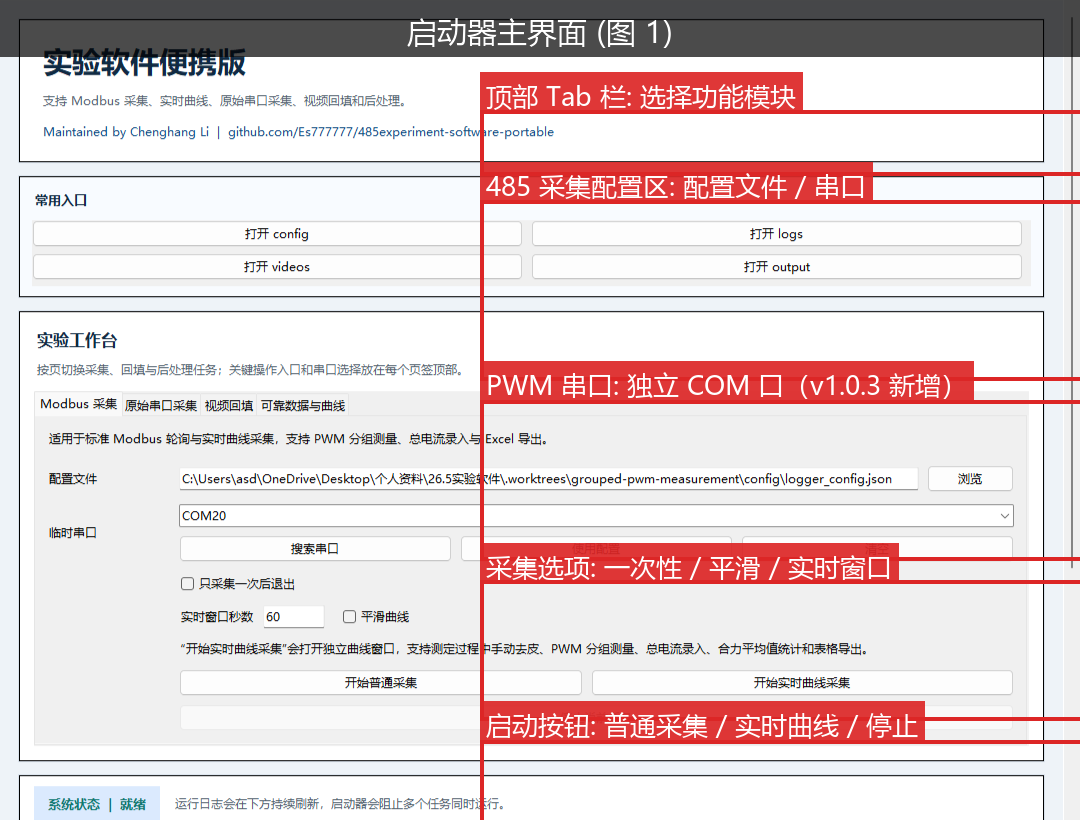
\includegraphics[width=0.94\textwidth]{manual_assets/annotated/launcher_main_annotated.png}
  \caption{启动器主界面（红色框标注：顶部 Tab 栏、功能模块说明区、快捷入口）}
\end{figure}

\subsection{第二步：确认串口与配置}

\begin{enumerate}[leftmargin=2em]
  \item 查看当前选中的配置文件；
  \item 确认串口号与设备管理器显示一致；
  \item 如果软件支持搜索串口，先点一次搜索，再选择实际设备；
  \item 如近期更换过传感器、采集板或固件版本，必须重新确认寄存器地址和字序。
\end{enumerate}

\textbf{经验建议：}只要出现“昨天正常、今天某一路数值特别怪”，先别怀疑力矩公式，先怀疑串口选错、设备没接对、配置没切对。

\subsection{第三步：打开实时曲线}

\begin{enumerate}[leftmargin=2em]
  \item 在启动器中点击“开始实时曲线采集”；
  \item 等待实时曲线窗口打开；
  \item 观察窗口顶部状态是否进入正常采集；
  \item 如果窗口打开失败，优先检查依赖、串口占用和权限问题。
\end{enumerate}

\begin{figure}[H]
  \centering
  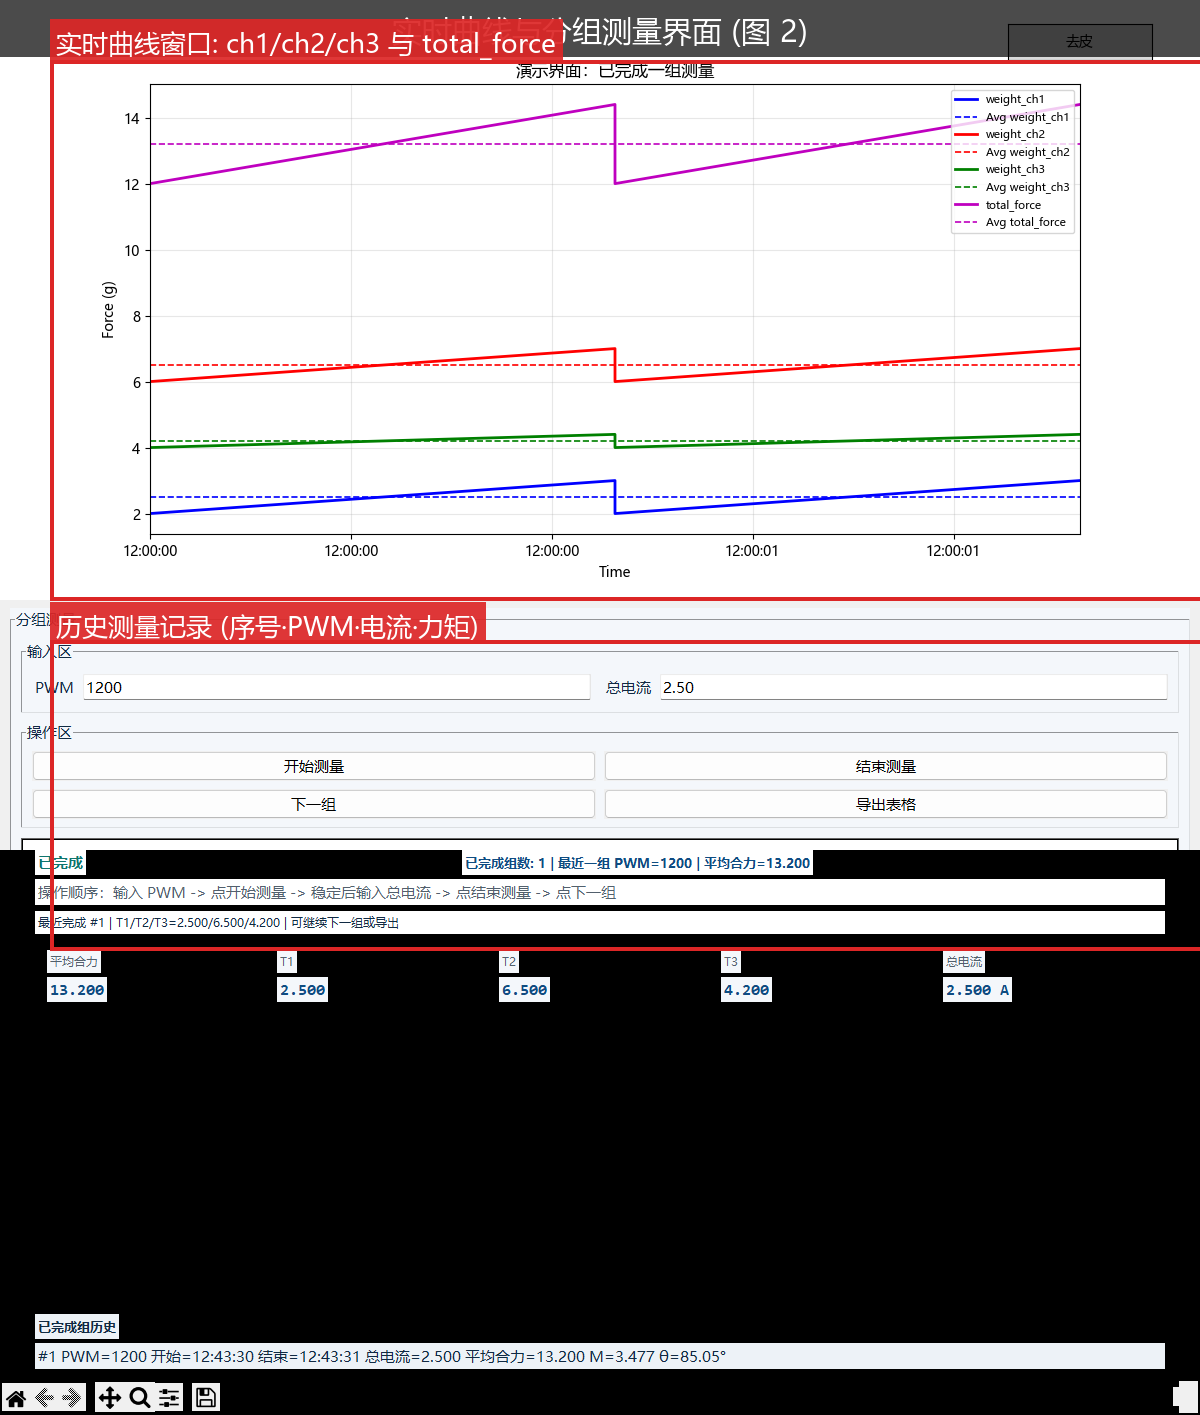
\includegraphics[width=0.92\textwidth]{manual_assets/annotated/live_plot_moment_panel_annotated.png}
  \caption{实时曲线与分组测量界面（红色框标注：实时曲线窗口、测量操作面板、历史测量记录）}
\end{figure}

\subsection{便携版（v1.0.4）使用说明}

便携版不依赖 Python，下载解压后即可运行：

\begin{enumerate}[leftmargin=2em]
  \item 在 GitHub Releases 页面下载
        \texttt{485experiment-software-portable-v1.0.4-20261013.zip}；
  \item 解压到任意目录（路径不要含中文或空格以外的特殊字符）；
  \item 双击 \texttt{实验软件.exe} 启动；
  \item 第一次启动若弹出权限提示，同意即可；
  \item “配置 / 日志 / 视频 / 输出”等快捷入口在启动器底部。
\end{enumerate}

\begin{figure}[H]
  \centering
  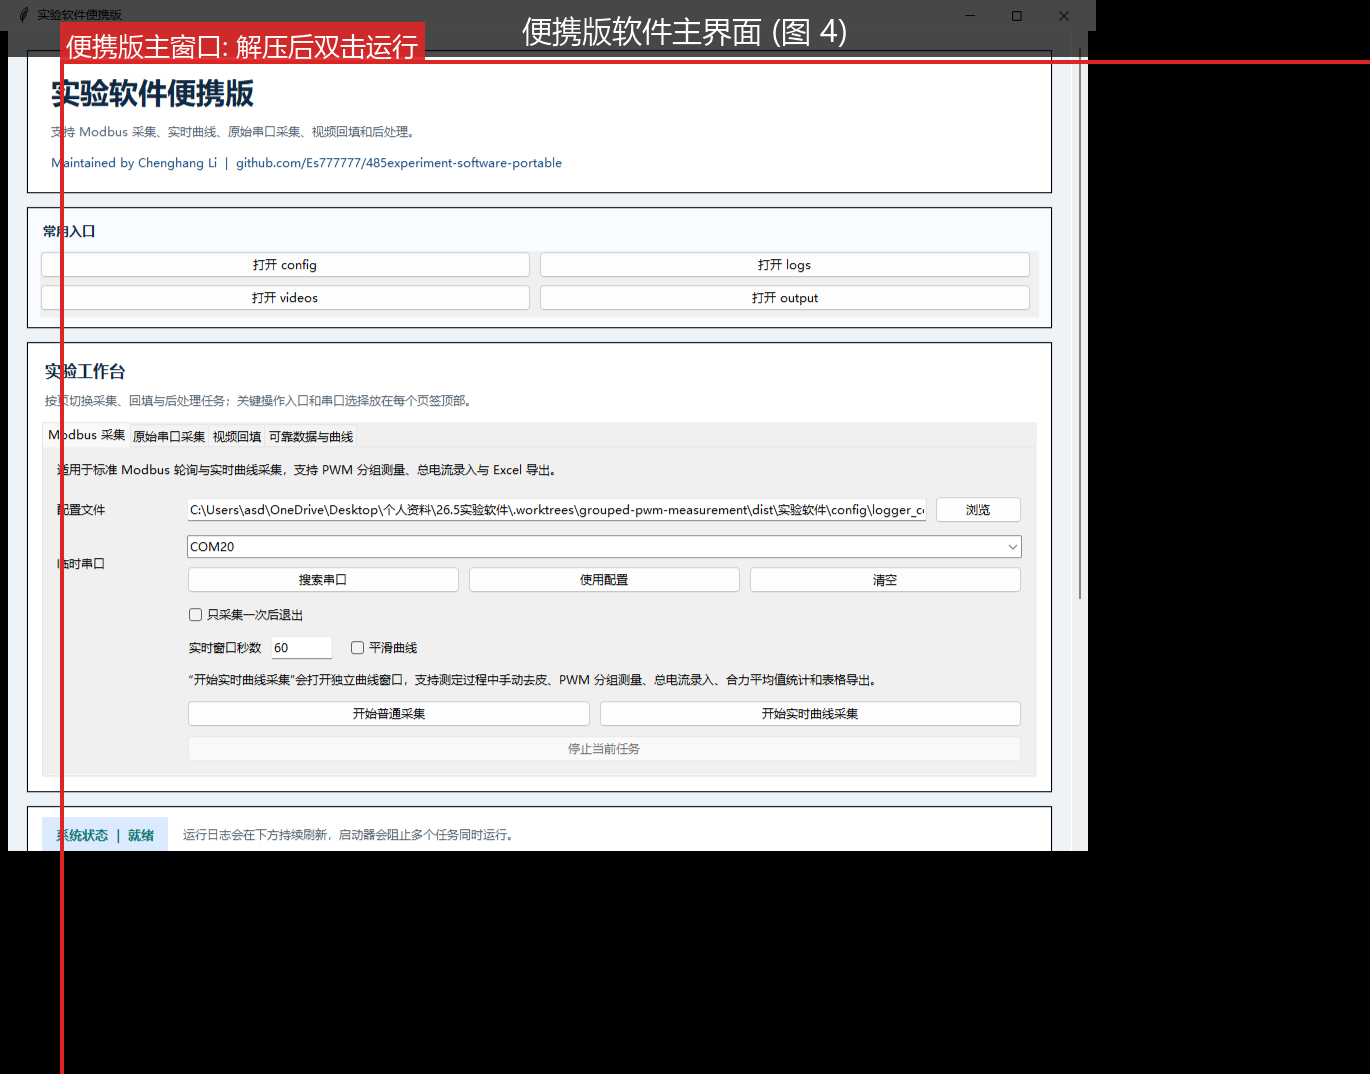
\includegraphics[width=0.94\textwidth]{manual_assets/annotated/portable_exe_main_annotated.png}
  \caption{便携版软件主界面（红色框标注：解压后双击运行的主窗口）}
\end{figure}

\subsection{问题反馈（v1.0.4 新增）}

启动器底部新增“问题反馈”页签，可将实验中发现的问题直接发到维护者邮箱。

\begin{enumerate}[leftmargin=2em]
  \item 切到“问题反馈”页签；
  \item 填写主题、邮箱（仅作回信展示，非必填）、问题正文；
  \item 点击“发送”；
  \item 发送前需在 \texttt{config/email.json} 写入发件邮箱 + QQ 邮箱授权码（不是登录密码），首次启动会提示；
  \item 同一邮箱每日最多 8 封、两次发送至少间隔 60 秒，避免邮箱被打爆。
\end{enumerate}

\textbf{注意：}授权码必须使用 QQ 邮箱“账户 $\rightarrow$ POP3/IMAP/SMTP/Exchange/CardDAV/CalDAV服务”页面申请的应用专用密码，不能填写登录密码。

\subsection{第四步：去皮}

\subsubsection{什么时候去皮}

推荐在以下场景去皮：
\begin{itemize}[leftmargin=2em]
  \item 软件刚启动；
  \item 装夹或加载状态变化后；
  \item 曲线整体偏离零点明显时；
  \item 换组前发现静止状态下三路通道基线已经漂移。
\end{itemize}

\subsubsection{怎么做}

\begin{enumerate}[leftmargin=2em]
  \item 确保传感器处于你希望定义为“零点”的稳定状态；
  \item 点击“去皮”；
  \item 不要在去皮过程中碰设备或施加额外扰动；
  \item 去皮完成后，再看 ch1/ch2/ch3 是否围绕新零点波动。
\end{enumerate}

\textbf{注意：}去皮不是“把错误数据修好”，它只是重新定义零点。如果寄存器读错、字序错或串口不对，去皮后仍然会错。

\subsection{第五步：观察曲线是否正常}

正常情况下，实时曲线应满足：

\begin{enumerate}[leftmargin=2em]
  \item 三路通道在静止时围绕某个稳定基线小幅波动；
  \item 总合力 \texttt{total\_force} 会随三路变化而同步变化；
  \item 人为加载时，相关通道有响应，卸载后能回落；
  \item 不应长期出现毫无规律的大幅乱跳；
  \item 不应每一路都完全一模一样。
\end{enumerate}

\section{曲线判读重点}

\subsection{ch1、ch2、ch3 与 total\_force 的关系}

\begin{itemize}[leftmargin=2em]
  \item \texttt{weight\_ch1}、\texttt{weight\_ch2}、\texttt{weight\_ch3}：三路单独通道；
  \item \texttt{total\_force}：三路通道求和后的合力；
  \item 因此 \texttt{total\_force} 本来就可能接近某一路的 2 倍或 3 倍；
  \item 如果把 \texttt{total\_force} 误当成某一路，会误以为“软件把某个通道乘大了”。
\end{itemize}

\subsection{什么情况值得怀疑配置有问题}

如果出现以下现象，应优先检查配置和硬件映射：

\begin{enumerate}[leftmargin=2em]
  \item 某一路长期明显大于另外两路，且不符合实验载荷分布；
  \item 某一路几乎总是另一条的固定倍数；
  \item 三路曲线形状完全一样，只是数值整体平移或放大；
  \item 数值偶尔突然跳到极大或极小值；
  \item 去皮后曲线仍然像“抽风”，没有稳定基线。
\end{enumerate}

\subsection{这时先查什么}

\begin{enumerate}[leftmargin=2em]
  \item 当前串口是不是接到了正确设备；
  \item \texttt{weight\_ch1/ch2/ch3} 地址是否还是 0、2、4；
  \item 当前设备是否仍然使用 \texttt{int32 + word\_order=little}；
  \item 最近是否换过板卡、固件或传感器；
  \item 是否把 \texttt{total\_force} 看成了单路通道。
\end{enumerate}

\section{PWM 分组测量操作}

\subsection{开始测量前}

\begin{enumerate}[leftmargin=2em]
  \item 先确认去皮已经完成；
  \item 曲线已经恢复稳定；
  \item 知道本组要记录的 PWM；
  \item 知道结束时要填写的总电流值。
\end{enumerate}

\subsection{开始一组}

\begin{enumerate}[leftmargin=2em]
  \item 在分组测量区域输入本组 \texttt{PWM}；
  \item 点击“开始测量”；
  \item 软件开始记录本组开始时间和后续采样。
\end{enumerate}

\subsection{采集中应该做什么}

\begin{enumerate}[leftmargin=2em]
  \item 观察三路曲线是否进入稳定区间；
  \item 如果这组实验存在明显过渡过程，不要太早结束；
  \item 尽量在稳定阶段内结束测量，保证导出的平均值有意义。
\end{enumerate}

\subsection{结束一组}

\begin{enumerate}[leftmargin=2em]
  \item 在“总电流”输入框填写本组实际总电流；
  \item 点击“结束测量”；
  \item 软件将计算：
  \begin{itemize}[leftmargin=2em]
    \item 平均合力
    \item \(T1\)、\(T2\)、\(T3\)
    \item \(M_y\)
    \item \(M_x\)
    \item \(M\)
    \item \(\theta\)
  \end{itemize}
\end{enumerate}

\subsection{看结果时重点看什么}

\begin{enumerate}[leftmargin=2em]
  \item 平均合力是否与曲线稳定区间大致一致；
  \item \(T1/T2/T3\) 是否符合载荷分配直觉；
  \item 力矩方向和大小是否符合实验姿态；
  \item 历史组记录中 PWM 和总电流是否填错。
\end{enumerate}

\begin{figure}[H]
  \centering
  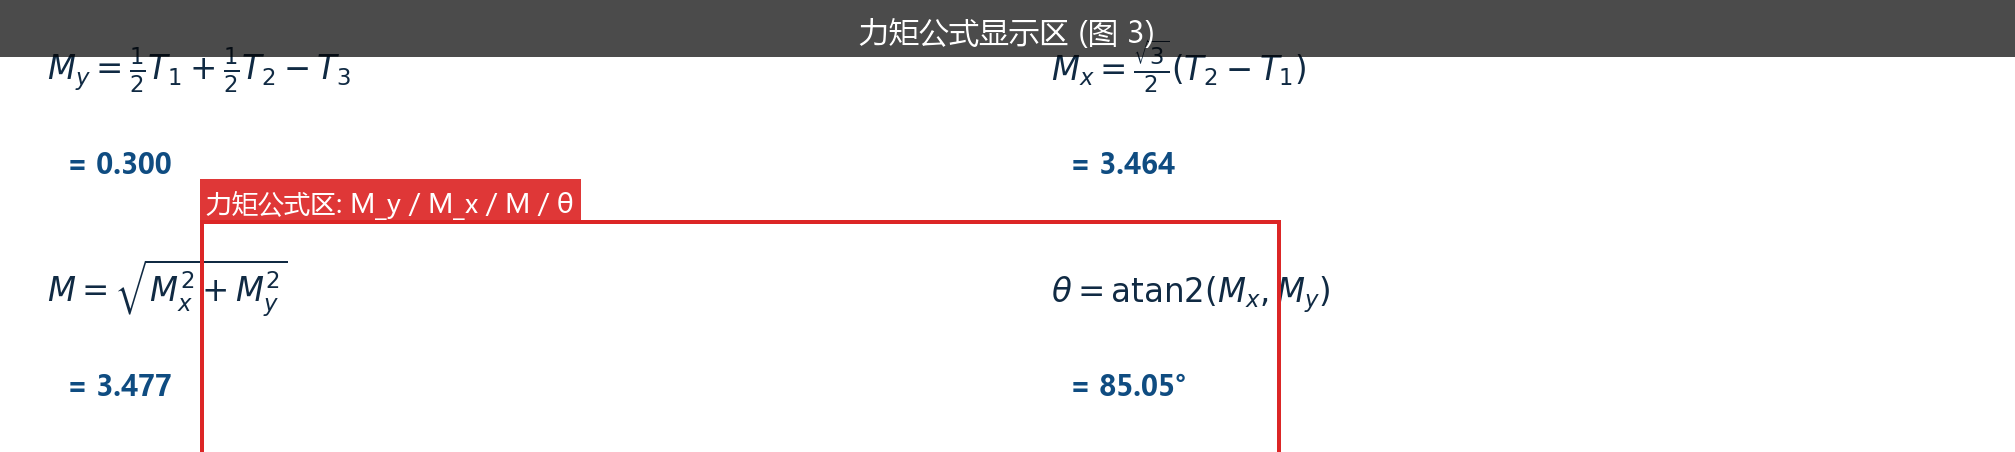
\includegraphics[width=0.9\textwidth]{manual_assets/annotated/moment_formula_panel_annotated.png}
  \caption{力矩公式显示区（红色框标注：$M_y$ / $M_x$ / $M$ / $\theta$ 公式区）}
\end{figure}

\subsection{进入下一组}

\begin{enumerate}[leftmargin=2em]
  \item 点击“下一组”；
  \item 确认当前组已进入历史；
  \item 重新输入下一组 PWM；
  \item 如零点已有漂移，可先重新去皮，再开始下一组。
\end{enumerate}

\subsection{导出表格}

\begin{enumerate}[leftmargin=2em]
  \item 所有组完成后点击“导出表格”；
  \item 导出文件默认写入 \texttt{output/}；
  \item 导出结果包含汇总列和原始采样列；
  \item 导出后建议立即打开检查是否成功生成。
\end{enumerate}

\section{导出结果怎么看}

\subsection{汇总列}

导出表前部通常包括：

\begin{itemize}[leftmargin=2em]
  \item 序号
  \item PWM
  \item 开始时间
  \item 结束时间
  \item 总电流
  \item 合力平均值
  \item T1 平均值
  \item T2 平均值
  \item T3 平均值
  \item \(M_y\)
  \item \(M_x\)
  \item \(M\)
  \item \(\theta\)
\end{itemize}

\subsection{原始列}

导出表后部还会保留每组内部采样的原始时间戳、原始合力和通道值，便于复核平均值来自哪一段数据。

\textbf{建议：}如果有人反馈“这一组结果离谱”，先回头看该组原始列，而不是直接看汇总值。

\section{常见异常与处理}

\subsection{现象一：软件能开，但实时曲线不显示}

优先检查：
\begin{enumerate}[leftmargin=2em]
  \item 是否打开的是旧版目录或旧版便携包；
  \item 串口是否成功连接；
  \item 当前电脑是否缺少图形依赖；
  \item 是否被其他串口工具占用。
\end{enumerate}

\subsection{现象二：ch1/ch2/ch3 像倍率不对或乱跳}

按下面顺序排查：

\begin{enumerate}[leftmargin=2em]
  \item 确认有没有把 \texttt{total\_force} 认成单路；
  \item 检查 \texttt{config/logger\_config.json} 地址与字序；
  \item 核对设备型号、固件版本和当前映射；
  \item 重新去皮；
  \item 观察静止状态下是否仍有大幅乱跳；
  \item 必要时保存日志和截图，回看原始采样。
\end{enumerate}

\subsection{现象三：导出失败}

优先检查：
\begin{enumerate}[leftmargin=2em]
  \item 导出的 Excel 是否已经被打开占用；
  \item \texttt{output/} 目录是否有写权限；
  \item 文件名是否冲突；
  \item 磁盘空间是否充足。
\end{enumerate}

\subsection{现象四：力矩结果和曲线直觉不一致}

优先检查：
\begin{enumerate}[leftmargin=2em]
  \item 去皮是否在正确状态下完成；
  \item 这组采样是否真的取自稳定区间；
  \item 三路通道是否存在明显异常值；
  \item 当前版本是否已经包含去皮一致性修复。
\end{enumerate}

\section{推荐操作习惯}

\begin{enumerate}[leftmargin=2em]
  \item 每次开机后先空载观察 5--10 秒；
  \item 每次正式测量前先去皮；
  \item 每组结束前确认曲线已经稳定；
  \item 导出后立刻检查文件是否真的写出；
  \item 遇到异常先截图，再改配置；
  \item 一旦更换硬件或固件，先重新核对寄存器映射。
\end{enumerate}

\section{本次更新内容（v1.0.4）}

本次更新相对 v1.0.4 主要增加了：

\begin{itemize}[leftmargin=2em]
  \item \textbf{双 COM 串口}：485 采集串口与 PWM 输出串口在代码与启动器中拆成
        两路独立 COM，可在 \texttt{config/logger\_config.json} 的
        \texttt{pwm.port} 字段里独立配置（也支持用启动器界面或
        \texttt{-\/-pwm-port} 命令行覆盖）；
  \item \textbf{PWM Modbus 写入}：分组测量输入的 PWM 实际通过功能码 06 写入
        \texttt{config/logger\_config.json} 中登记的寄存器；优先走独立 PWM 串口，
        未配置时回退到 485 总线（兼容旧设备）；
  \item \textbf{PWM 列写入主表}：主 live data 的 Excel 末尾新增 \texttt{pwm} 列；
  \item \textbf{统一 xlsx 导出}：分组测量结果与主数据共用同一份 Excel
        （\texttt{data} + \texttt{measurements} 两个 sheet）；
  \item \textbf{线程修复}：串口读取在 daemon 线程中执行，UI 走 Tk \texttt{after()} 调度，
        画布用 \texttt{draw\_idle()} 替换 \texttt{plt.pause}；
  \item \textbf{问题反馈邮件}：内置“问题反馈”页签，通过 QQ SMTP 发到
        \texttt{koji3527@qq.com}，每日上限 8 封、间隔 60 秒；
  \item \textbf{设备管理器排查章节}：本说明书新增“串口选型（双 COM）与设备管理器排查”章节，
        详细列出在设备管理器中如何识别两个 COM 编号以及如何处理串口占用问题；
  \item 真实页面截图 + 红色框 + 中文标注，所有 4 张关键截图（启动器、实时曲线、力矩公式、便携版主窗口）均更新为带标注的版本。
\end{itemize}

\section{本次生成文件}

\begin{itemize}[leftmargin=2em]
  \item \texttt{实验软件说明书\_20260705.tex}
  \item \texttt{实验软件说明书\_20260705.pdf}
  \item \texttt{manual\_assets/screenshots/launcher\_main.png}
  \item \texttt{manual\_assets/screenshots/live\_plot\_moment\_panel.png}
  \item \texttt{manual\_assets/screenshots/moment\_formula\_panel.png}
  \item \texttt{manual\_assets/screenshots/portable\_exe\_main.png}
  \item \texttt{manual\_assets/annotate\_screenshots.py}
  \item \texttt{manual\_assets/annotated/launcher\_main\_annotated.png}
  \item \texttt{manual\_assets/annotated/live\_plot\_moment\_panel\_annotated.png}
  \item \texttt{manual\_assets/annotated/moment\_formula\_panel\_annotated.png}
  \item \texttt{manual\_assets/annotated/portable\_exe\_main\_annotated.png}
  \item \texttt{RELEASE\_NOTES\_v1.0.4.md}
\end{itemize}

\end{document}
